\chapter{As moléculas orgânicas: esqueletos e nomes}\label{ch:g11:organic-skeletons}

Um isqueiro descartável contém butano, líquido sob pressão; o cartucho
de um fogareiro de camping levado para uma montanha nevada contém
propano, ou uma \omterm{def:g6:pure-substances-and-mixtures:mixture}{mistura} mais rica nele. Os dois são feitos só de \omterm{def:g7:atoms-and-molecules:atom}{átomos}
de carbono e de hidrogênio, e os dois pertencem a uma família enorme: as
\omterm{def:g7:atoms-and-molecules:molecule}{moléculas} construídas sobre um esqueleto de \omterm{def:g7:atoms-and-molecules:atom}{átomos} de carbono. São
conhecidas milhões delas. Para falar delas, os químicos precisam de
jeitos de desenhá-las depressa e de dar nomes a elas sem ambiguidade.

\begin{recall}
O carbono forma quatro \omterm{def:g10:lewis-and-shape:covalent-bond}{ligações covalentes} e o hidrogênio uma; em volta
de um \omterm{def:g7:atoms-and-molecules:atom}{átomo} de carbono com quatro ligações simples, as ligações apontam
para os vértices de um tetraedro, a cerca de \ang{109.5}
(\cref{ch:g10:lewis-and-shape}).
\end{recall}

\begin{omfigure}
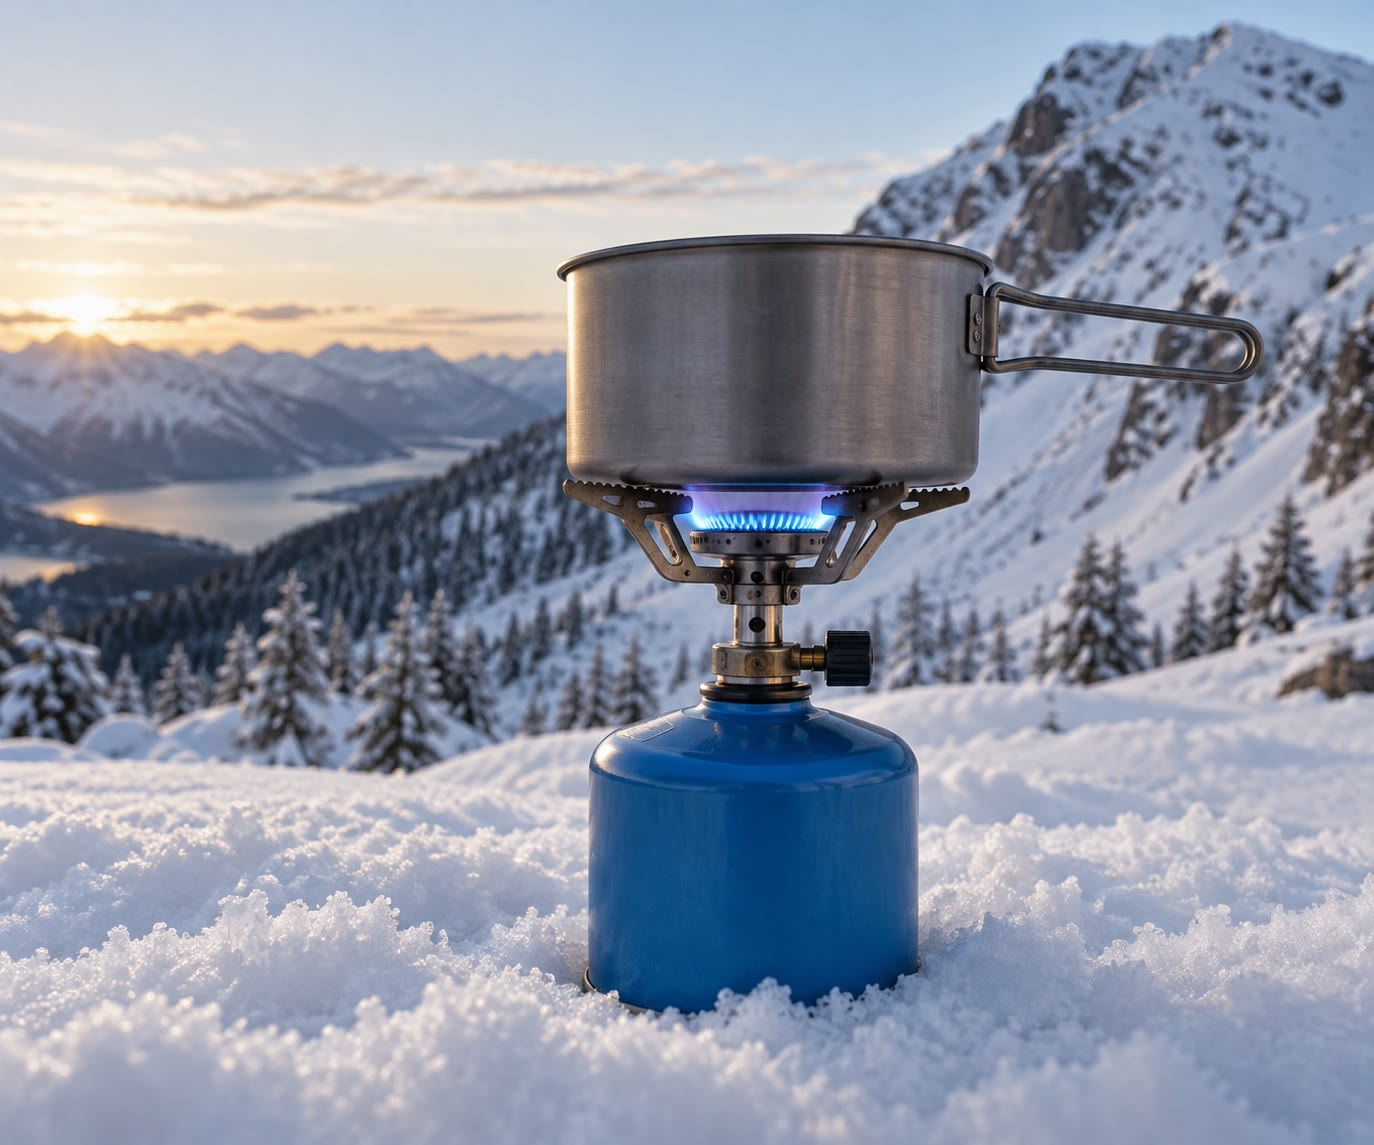
\includegraphics[width=0.48\linewidth]{images/book1/ai/g11-camping-cartridge.jpg}

{\small Um fogareiro de camping na neve, queimando um gás feito de
carbono e hidrogênio.}
\end{omfigure}

\section{As fórmulas das moléculas orgânicas}

\begin{definition}[Composto orgânico]\label{def:g11:organic-skeletons:organic}
Um \emph{composto orgânico}\index{composto organico@composto orgânico} é um composto cujas
\omterm{def:g7:atoms-and-molecules:molecule}{moléculas} são construídas sobre um esqueleto de \omterm{def:g7:atoms-and-molecules:atom}{átomos} de carbono
ligados entre si e a \omterm{def:g7:atoms-and-molecules:atom}{átomos} de hidrogênio, podendo ter outros \omterm{def:g7:atoms-and-molecules:atom}{átomos},
como o oxigênio e o nitrogênio. (O dióxido de carbono, o monóxido de
carbono e os carbonatos são tradicionalmente deixados de fora.)
\end{definition}

\begin{definition}[Quatro tipos de fórmula]\label{def:g11:organic-skeletons:formulas}
Uma \omterm{def:g7:atoms-and-molecules:molecule}{molécula} pode ser escrita de quatro jeitos:
\begin{itemize}
  \item a sua \emph{fórmula molecular}\index{formula molecular@fórmula molecular} dá só o
        número de \omterm{def:g7:atoms-and-molecules:atom}{átomos} de cada elemento, como \ce{C4H10};
  \item a sua \emph{fórmula estrutural}\index{formula estrutural@fórmula estrutural} mostra
        todos os \omterm{def:g7:atoms-and-molecules:atom}{átomos} e todas as ligações;
  \item a sua \emph{fórmula estrutural
        condensada}\index{formula estrutural condensada@fórmula estrutural condensada} mostra as
        ligações entre os \omterm{def:g7:atoms-and-molecules:atom}{átomos} de carbono e agrupa os \omterm{def:g7:atoms-and-molecules:atom}{átomos} de
        hidrogênio com o seu carbono, como \ce{CH3-CH2-CH2-CH3};
  \item a sua \emph{fórmula em bastão}\index{formula em bastao@fórmula em bastão} desenha só
        as ligações do esqueleto de carbono como um zigue-zague: cada
        extremidade e cada vértice é um \omterm{def:g7:atoms-and-molecules:atom}{átomo} de carbono, os \omterm{def:g7:atoms-and-molecules:atom}{átomos} de
        hidrogênio ligados ao carbono não são desenhados, e todos os
        outros \omterm{def:g7:atoms-and-molecules:atom}{átomos} (com os seus \omterm{def:g7:atoms-and-molecules:atom}{átomos} de hidrogênio) são escritos.
\end{itemize}
\end{definition}

\begin{omfigure}
\setchemfig{atom sep=1.45em}
\renewcommand{\arraystretch}{1.6}
\small
\begin{tabular}{@{}l@{\quad}c@{\quad}c@{}}
 & butano & 2-metilpropano \\
molecular & \ce{C4H10} & \ce{C4H10} \\[4pt]
estrutural &
\chemfig{H-C(-[2]H)(-[6]H)-C(-[2]H)(-[6]H)-C(-[2]H)(-[6]H)-C(-[2]H)(-[6]H)-H} &
\chemfig{H-C(-[2]H)(-[6]H)-C(-[6]H)(-[2,1.5]C(-[1]H)(-[3]H)(-[2]H))-C(-[2]H)(-[6]H)-H} \\[10pt]
condensada & \ce{CH3-CH2-CH2-CH3} &
\chemfig{CH_3-CH(-[6]CH_3)-CH_3} \\[14pt]
em bastão & \chemfig{-[:30]-[:-30]-[:30]} & \chemfig{-[:30](-[:90])-[:-30]} \\
\end{tabular}

{\small As quatro fórmulas do butano e do 2-metilpropano. Nas \omterm{def:g11:organic-skeletons:formulas}{fórmulas
em bastão}, cada extremidade e cada vértice das linhas é um \omterm{def:g7:atoms-and-molecules:atom}{átomo} de
carbono: quatro em cada uma.}
\end{omfigure}


\begin{example}[Ler uma fórmula em bastão]\label{ex:g11:organic-skeletons:reading}
Na \omterm{def:g11:organic-skeletons:formulas}{fórmula em bastão} do butano, o zigue-zague tem duas extremidades e
dois vértices: quatro \omterm{def:g7:atoms-and-molecules:atom}{átomos} de carbono. Cada carbono de extremidade tem
uma ligação desenhada, por isso leva três \omterm{def:g7:atoms-and-molecules:atom}{átomos} de hidrogênio
(\ce{CH3}); cada vértice tem duas ligações desenhadas, por isso leva dois
(\ce{CH2}). Todo carbono tem quatro ligações ao todo, o que devolve
\ce{C4H10}.
\end{example}

\section{As cadeias carbônicas}

O esqueleto de carbono de uma \omterm{def:g7:atoms-and-molecules:molecule}{molécula} pode ser uma cadeia
\emph{linear}, cada carbono ligado a no máximo dois outros, como no
butano; uma cadeia \emph{ramificada}, com pelo menos um carbono ligado a
três ou quatro outros, como no 2-metilpropano; ou um \emph{anel}, como
no ciclo-hexano, \ce{C6H12}, cuja \omterm{def:g11:organic-skeletons:formulas}{fórmula em bastão} é um hexágono. Usa-se
um zigue-zague para as cadeias porque as ligações reais em volta de cada
carbono formam ângulos de cerca de \ang{109.5}, e não de \ang{180}: uma
cadeia ``linear'' é na verdade um zigue-zague no espaço.
\begin{omfigure}
\setchemfig{atom sep=1.9em}
\begin{tabular}{ccc}
\chemfig{-[:30]-[:-30]-[:30]-[:-30]-[:30]} &
\chemfig{-[:30](-[:90])-[:-30]-[:30](-[:90])-[:-30]} &
\chemfig{*6(------)} \\[4pt]
\small linear: hexano & \small ramificada: 2,4-dimetilpentano &
\small anel: ciclo-hexano \\
\small \ce{C6H14} & \small \ce{C7H16} & \small \ce{C6H12}
\end{tabular}

{\small Três esqueletos de carbono, em \omterm{def:g11:organic-skeletons:formulas}{fórmulas em bastão}.}
\end{omfigure}

\section{Os alcanos e os seus nomes}

\begin{definition}[Alcano, grupo alquila]\label{def:g11:organic-skeletons:alkane}
Um \emph{alcano}\index{alcano} é um composto de carbono e hidrogênio cujo
esqueleto é uma cadeia (linear ou ramificada, não um anel) só com
ligações simples; a sua \omterm{def:g11:organic-skeletons:formulas}{fórmula molecular} é \ce{C_{n}H_{2n+2}}. Um
\emph{grupo alquila}\index{grupo alquila} é o que sobra de um alcano
quando se retira um \omterm{def:g7:atoms-and-molecules:atom}{átomo} de hidrogênio, para que ele possa ser ligado a
uma cadeia: metil \ce{-CH3}, etil \ce{-CH2-CH3}.
\end{definition}

\begin{omfigure}
\begin{tabular}{rlcrlc}
\hline
$n$ & nome & fórmula & $n$ & nome & fórmula \\
\hline
1 & metano & \ce{CH4}    & 6  & hexano & \ce{C6H14} \\
2 & etano  & \ce{C2H6}   & 7  & heptano & \ce{C7H16} \\
3 & propano & \ce{C3H8}   & 8  & octano & \ce{C8H18} \\
4 & butano  & \ce{C4H10}  & 9  & nonano & \ce{C9H20} \\
5 & pentano & \ce{C5H12}  & 10 & decano & \ce{C10H22} \\
\hline
\end{tabular}\par\medskip

{\small Os dez primeiros \omterm{def:g11:organic-skeletons:alkane}{alcanos} lineares. O nome de uma cadeia de $n$
\omterm{def:g7:atoms-and-molecules:atom}{átomos} de carbono é o mesmo radical seguido de \emph{-ano}; o \omterm{def:g11:organic-skeletons:alkane}{grupo
alquila} troca \emph{-ano} por \emph{-il} (metil, etil, propil\dots).}
\end{omfigure}

\begin{method}[Dar nome a um alcano]\label{met:g11:organic-skeletons:naming}
\begin{enumerate}
  \item Encontre a cadeia mais longa de \omterm{def:g7:atoms-and-molecules:atom}{átomos} de carbono: ela dá o nome
        de base (pentano, hexano\dots).
  \item Os \omterm{def:g7:atoms-and-molecules:atom}{átomos} que não estão nela formam \omterm{def:g11:organic-skeletons:alkane}{grupos alquila} ligados a
        ela, os substituintes.
  \item Numere a cadeia principal a partir da extremidade que dá aos
        substituintes os menores números.
  \item Escreva cada substituinte com o seu número (a sua posição na
        cadeia), em ordem alfabética, antes do nome de base; os grupos
        repetidos levam os prefixos di-, tri-, tetra-, com um número para
        cada um. Os números são separados por vírgulas, e os números e
        as palavras por hífens.
\end{enumerate}
\end{method}

\begin{omfigure}
\begin{tikzpicture}[font=\small, x=0.9cm, y=0.9cm]
  % main chain of 5, zigzag; methyls on C2 and C3
  \coordinate (a1) at (0,0); \coordinate (a2) at (0.87,0.5);
  \coordinate (a3) at (1.73,0); \coordinate (a4) at (2.6,0.5);
  \coordinate (a5) at (3.46,0);
  \coordinate (m2) at (0.87,1.5); \coordinate (m3) at (1.73,-1);
  \draw[line width=1pt] (a1) -- (a2) -- (a3) -- (a4) -- (a5);
  \draw[line width=1pt] (a2) -- (m2); \draw[line width=1pt] (a3) -- (m3);
  \foreach \k in {1,2,3,4,5}
    \node[omDef, font=\footnotesize\bfseries, fill=white, inner sep=1pt]
      at ($(a\k)+(0,-0.32)$) {\k};
  \draw[omProp, thick] (m2) circle (0.28);
  \draw[omProp, thick] (m3) circle (0.28);
  \node[omProp, anchor=west] at ($(m2)+(0.35,0)$) {metil no C2};
  \node[omProp, anchor=west] at ($(m3)+(0.35,0)$) {metil no C3};
  \node[anchor=west, align=left] at (5,0.3) {cadeia mais longa: 5 carbonos,
    \emph{pentano}\\ numerada pela esquerda: 2 e 3\\ (pela direita: 3
    e 4, maiores)\\ nome: \textbf{2,3-dimetilpentano}};
\end{tikzpicture}

{\small Dar nome a um \omterm{def:g11:organic-skeletons:alkane}{alcano} ramificado: a cadeia principal (numerada),
os substituintes (circulados), o nome.}
\end{omfigure}

\begin{method}[De um nome a uma fórmula em bastão]\label{met:g11:organic-skeletons:drawing}
\begin{enumerate}
  \item Desenhe a cadeia principal dada pelo nome de base, como um
        zigue-zague, e numere os seus carbonos.
  \item Ligue cada substituinte na posição dada pelo seu número.
  \item Verifique: conte os carbonos, e veja se nenhum carbono tem mais
        de quatro ligações.
\end{enumerate}
\end{method}

\section{Os isômeros}

\begin{definition}[Isômeros, isômeros constitucionais]\label{def:g11:organic-skeletons:isomer}
\emph{Isômeros}\index{isomeros@isômeros} são compostos diferentes com a mesma
\omterm{def:g11:organic-skeletons:formulas}{fórmula molecular}. \emph{Isômeros constitucionais}\index{isomeros constitucionais@isômeros constitucionais}
são isômeros cujos \omterm{def:g7:atoms-and-molecules:atom}{átomos} estão ligados numa ordem diferente, por exemplo com um esqueleto de carbono diferente.
\end{definition}

\begin{proposition}[Os isômeros têm propriedades diferentes]\label{prop:g11:organic-skeletons:properties}
% ledger: bp:C4H10, bp:isobutane, bp:C5H12, bp:isopentane, bp:neopentane
Os \omterm{def:g11:organic-skeletons:isomer}{isômeros constitucionais} são substâncias diferentes, com propriedades
diferentes. Entre os \omterm{def:g11:organic-skeletons:alkane}{alcanos} \omterm{def:g11:organic-skeletons:isomer}{isômeros} de uma dada fórmula, os mais
ramificados fervem a temperaturas mais baixas: o butano ferve perto de
\qty{0}{\celsius} e o 2-metilpropano a \qty{-11.7}{\celsius}; o pentano
a \qty{36.1}{\celsius}, o 2-metilbutano a \qty{27.8}{\celsius} e o
2,2-dimetilpropano a \qty{9.5}{\celsius}.
\end{proposition}

\begin{proof}
Os valores são medidos. As \omterm{def:g7:atoms-and-molecules:molecule}{moléculas} ramificadas são
mais compactas, com menos superfície em contato com as vizinhas: as suas
\omterm{def:g11:polarity-and-cohesion:van-der-waals}{interações de van der Waals} são mais fracas
(\cref{ch:g11:polarity-and-cohesion}).
\end{proof}

\begin{omfigure}
\setchemfig{atom sep=2em}
\begin{tabular}{ccc}
\chemfig{-[:30]-[:-30]-[:30]-[:-30]} &
\chemfig{-[:30](-[:90])-[:-30]-[:30]} &
\chemfig{-[:0](-[:90])(-[:-90])-[:0]} \\[24pt]
\small pentano & \small 2-metilbutano & \small 2,2-dimetilpropano \\
\small \qty{36.1}{\celsius} & \small \qty{27.8}{\celsius} &
\small \qty{9.5}{\celsius}
\end{tabular}
\medskip

{\small Os três \omterm{def:g11:organic-skeletons:isomer}{isômeros} de \ce{C5H12} e as suas temperaturas de
ebulição: quanto mais ramificado, mais baixa.}
\end{omfigure}

\section{Os alcanos do petróleo}

O petróleo bruto é uma \omterm{def:g6:pure-substances-and-mixtures:mixture}{mistura} de milhares de compostos, a maioria deles
\omterm{def:g11:organic-skeletons:alkane}{alcanos} com de 1 a mais de 40 \omterm{def:g7:atoms-and-molecules:atom}{átomos} de carbono. Numa refinaria, ele é
aquecido, e os seus vapores sobem por uma coluna alta, cada vez mais
fria em direção ao topo: cada fração se condensa na altura em que a
temperatura corresponde à sua faixa de ebulição. Os gases (do metano ao
butano) saem no topo, depois a gasolina, o querosene, o óleo diesel; os
óleos pesados e o betume ficam embaixo. Essa \omterm{def:g10:chemical-species:distillation}{destilação} fracionada
separa pela temperatura de ebulição, que, nos \omterm{def:g11:organic-skeletons:alkane}{alcanos}, cresce com o
comprimento da cadeia.

\begin{omfigure}
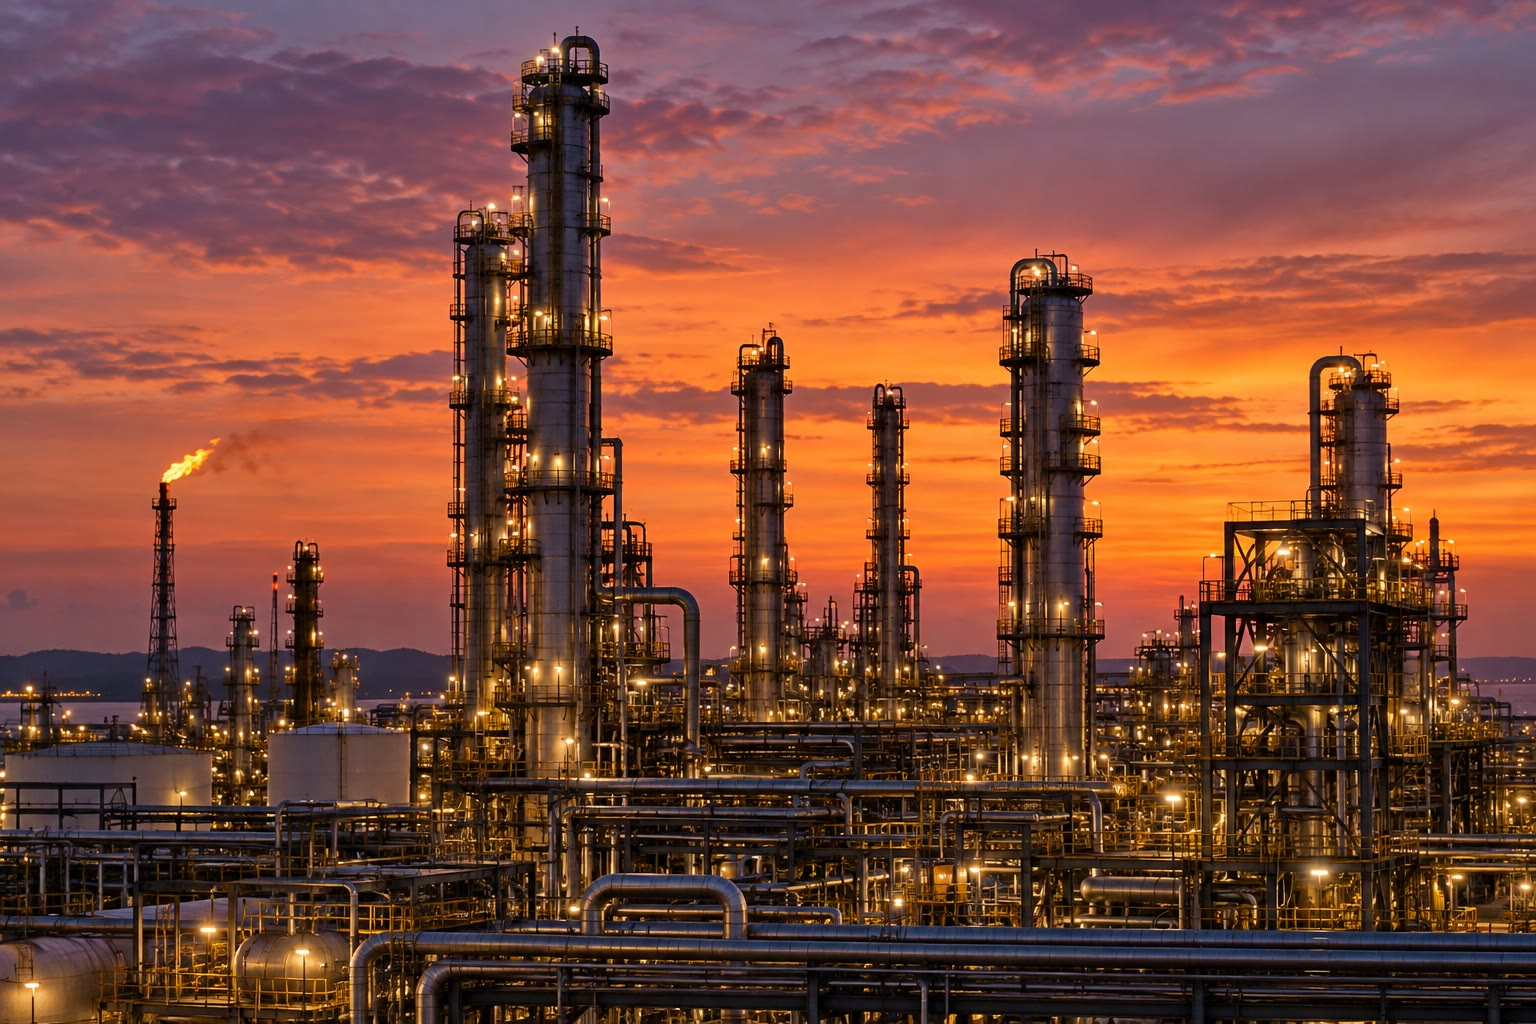
\includegraphics[width=0.52\linewidth]{images/book1/ai/g11-refinery-dusk.jpg}

{\small Colunas de \omterm{def:g10:chemical-species:distillation}{destilação} de uma refinaria ao entardecer.}
\end{omfigure}

\begin{safety}{\ghs[0.66cm]{GHS02}\ghs[0.66cm]{GHS04}\ghs[0.66cm]{GHS07}\ghs[0.66cm]{GHS08}\ghs[0.66cm]{GHS09}}
% ledger: ghs:butane, ghs:pentane
O butano é um gás extremamente inflamável, guardado sob pressão. O
pentano é um líquido altamente inflamável; o seu vapor provoca
sonolência, ele pode lesar os pulmões se ingerido e é tóxico para os
organismos aquáticos. Nenhuma chama perto dos \omterm{def:g11:organic-skeletons:alkane}{alcanos} leves; trabalhar
numa capela de exaustão.
\end{safety}

\section{Exercícios}


\begin{exercise}[$\star$]\label{exo:g11:organic-skeletons:1}
Dê as \omterm{def:g11:organic-skeletons:formulas}{fórmulas moleculares} das \omterm{def:g7:atoms-and-molecules:molecule}{moléculas} desenhadas aqui, e diga se elas
são isômeras:
\setchemfig{atom sep=1.6em}
\chemfig{-[:30]-[:-30]-[:30]-[:-30]-[:30]} \quad e \quad
\chemfig{-[:30](-[:90])-[:-30]-[:30]-[:-30]}.
\end{exercise}

\begin{exercise}[$\star$]\label{exo:g11:organic-skeletons:2}
Dê o nome: \ce{CH3-CH2-CH3}; \ce{CH3-CH2-CH2-CH2-CH2-CH3};
\chemfig{CH_3-CH(-[2]CH_3)-CH_2-CH_3}.
\end{exercise}

\begin{exercise}[$\star$]\label{exo:g11:organic-skeletons:3}
Escreva as \omterm{def:g11:organic-skeletons:formulas}{fórmulas estruturais condensadas} do propano e do
2-metilpropano, e a \omterm{def:g11:organic-skeletons:formulas}{fórmula estrutural} do etano.
\end{exercise}

\begin{exercise}[$\star$]\label{exo:g11:organic-skeletons:4}
Conte os \omterm{def:g7:atoms-and-molecules:atom}{átomos} de carbono e de hidrogênio de cada \omterm{def:g7:atoms-and-molecules:molecule}{molécula}:
\setchemfig{atom sep=1.6em}
\chemfig{-[:30]-[:-30](-[:-90])-[:30]-[:-30]} \quad e \quad
\chemfig{*6(------)}.
\end{exercise}

\begin{exercise}[$\star$]\label{exo:g11:organic-skeletons:5}
Dê a \omterm{def:g11:organic-skeletons:formulas}{fórmula molecular} do \omterm{def:g11:organic-skeletons:alkane}{alcano} com 8 \omterm{def:g7:atoms-and-molecules:atom}{átomos} de carbono, e o número de
\omterm{def:g7:atoms-and-molecules:atom}{átomos} de carbono do \omterm{def:g11:organic-skeletons:alkane}{alcano} com 20 \omterm{def:g7:atoms-and-molecules:atom}{átomos} de hidrogênio.
\end{exercise}

\begin{exercise}[$\star\star$]\label{exo:g11:organic-skeletons:6}
Desenhe as \omterm{def:g11:organic-skeletons:formulas}{fórmulas em bastão} do 3-metil-hexano, do 2,2-dimetilbutano e
do 3-etilpentano, e dê as suas \omterm{def:g11:organic-skeletons:formulas}{fórmulas moleculares}.
\end{exercise}

\begin{exercise}[$\star\star$]\label{exo:g11:organic-skeletons:7}
Desenhe e dê o nome dos três \omterm{def:g11:organic-skeletons:isomer}{isômeros} de \ce{C5H12}.
\end{exercise}

\begin{exercise}[$\star\star$]\label{exo:g11:organic-skeletons:8}
Estes nomes estão errados. Desenhe cada \omterm{def:g7:atoms-and-molecules:molecule}{molécula} e dê o seu nome certo:
2-etilbutano; 4-metilpentano; 1-metilbutano.
\end{exercise}

\begin{exercise}[$\star\star$]\label{exo:g11:organic-skeletons:9}
Usando a figura dos \omterm{def:g11:organic-skeletons:isomer}{isômeros} de \ce{C5H12}, ordene-os por temperatura
de ebulição e explique a ordem.
\end{exercise}

\begin{exercise}[$\star\star$]\label{exo:g11:organic-skeletons:10}
O ciclo-hexano é \ce{C6H12} e o hexano \ce{C6H14}. Explique os dois
\omterm{def:g7:atoms-and-molecules:atom}{átomos} de hidrogênio que faltam. Os dois compostos são \omterm{def:g11:organic-skeletons:isomer}{isômeros}? O
ciclo-hexano é um \omterm{def:g11:organic-skeletons:alkane}{alcano}?
\end{exercise}

\begin{exercise}[$\star\star$]\label{exo:g11:organic-skeletons:11}
Entre o propano, o butano, o 2-metilpropano e o ciclobutano (\ce{C4H8},
um anel de quatro \omterm{def:g7:atoms-and-molecules:atom}{átomos} de carbono), quais são \omterm{def:g11:organic-skeletons:isomer}{isômeros} entre si?
\end{exercise}

\begin{exercise}[$\star\star\star$]\label{exo:g11:organic-skeletons:12}
Desenhe e dê o nome dos cinco \omterm{def:g11:organic-skeletons:isomer}{isômeros} de \ce{C6H14}.
\end{exercise}

\begin{exercise}[$\star\star\star$]\label{exo:g11:organic-skeletons:13}
Imagine um \omterm{def:g11:organic-skeletons:alkane}{alcano} linear como um longo zigue-zague e um \omterm{def:g11:organic-skeletons:alkane}{alcano} muito
ramificado como uma bola. Usando essa imagem, explique por que a
ramificação abaixa a temperatura de ebulição dos \omterm{def:g11:organic-skeletons:isomer}{isômeros}.
\end{exercise}

\begin{exercise}[$\star\star\star$]\label{exo:g11:organic-skeletons:14}
Dê o nome do \omterm{def:g11:organic-skeletons:alkane}{alcano}
\begin{center}
\chemfig{CH_3-CH(-[2]CH_3)-CH_2-C(-[2]CH_3)(-[6]CH_3)-CH_2-CH_3}
\end{center}
\end{exercise}

\begin{exercise}[$\star\star\star$]\label{exo:g11:organic-skeletons:15}
O composto de referência da gasolina, o ``isoctano'', é o
2,2,4-trimetilpentano. Desenhe a sua \omterm{def:g11:organic-skeletons:formulas}{fórmula em bastão}, verifique que ele
é um \omterm{def:g11:organic-skeletons:isomer}{isômero} do octano, e escreva a sua \omterm{def:g11:organic-skeletons:formulas}{fórmula estrutural condensada}.
\end{exercise}

\section{Problema: o gás do isqueiro}

\begin{problem}[{Problema de fim de semana --- quantos \omterm{def:g11:organic-skeletons:alkane}{alcanos} diferentes
têm a fórmula \ce{C7H16}?}]
\label{pb:g11:organic-skeletons:1}
% ledger: bp:C3H8, bp:C4H10, bp:isobutane
Um isqueiro contém butano; um cartucho de camping de inverno contém uma
\omterm{def:g6:pure-substances-and-mixtures:mixture}{mistura} mais rica em propano ou em 2-metilpropano. O butano ferve a
cerca de \qty{0}{\celsius}, o 2-metilpropano a \qty{-11.7}{\celsius} e o
propano a \qty{-42}{\celsius}.

\medskip
\noindent\textbf{Parte I --- Dois gases com uma mesma fórmula.}
\begin{enumerate}
  \item Dê a \omterm{def:g11:organic-skeletons:formulas}{fórmula molecular} do butano, e verifique que ela segue a
        fórmula geral dos \omterm{def:g11:organic-skeletons:alkane}{alcanos}.
  \item Desenhe a sua \omterm{def:g11:organic-skeletons:formulas}{fórmula estrutural}.
  \item Escreva a sua \omterm{def:g11:organic-skeletons:formulas}{fórmula estrutural condensada} e a sua \omterm{def:g11:organic-skeletons:formulas}{fórmula em
        bastão}.
  \item Desenhe o 2-metilpropano dos mesmos três jeitos. Por que ele tem
        a mesma \omterm{def:g11:organic-skeletons:formulas}{fórmula molecular}?
  \item O butano e o 2-metilpropano são \omterm{def:g11:organic-skeletons:isomer}{isômeros}? De que tipo?
\end{enumerate}

\medskip
\noindent\textbf{Parte II --- No frio.}
\begin{enumerate}[resume]
  \item Quais dos três gases são gases a \qty{20}{\celsius} e à pressão
        normal?
  \item Um isqueiro aberto é usado ao \omterm{def:g4:air-a-mixture-of-gases:air}{ar} livre a \qty{-5}{\celsius}. Por
        que ele dá uma chama fraca?
  \item Por que os cartuchos de inverno são ricos em propano ou em
        2-metilpropano?
  \item Explique por que o 2-metilpropano ferve a uma temperatura mais
        baixa que o butano.
  \item Por que o propano não tem \omterm{def:g11:organic-skeletons:isomer}{isômero}?
\end{enumerate}

\medskip
\noindent\textbf{Parte III --- Dar nomes e contar.}
\begin{enumerate}[resume]
  \item Dê o nome de \chemfig{CH_3-CH(-[2]CH_3)-CH_2-CH_3}.
  \item Por que o nome ``3-metilbutano'' está errado para a mesma
        \omterm{def:g7:atoms-and-molecules:molecule}{molécula}?
  \item Quantos \omterm{def:g11:organic-skeletons:alkane}{alcanos} \omterm{def:g11:organic-skeletons:isomer}{isômeros} têm as fórmulas \ce{C4H10},
        \ce{C5H12} e \ce{C6H14}?
\end{enumerate}

\medskip
\noindent\textbf{Parte IV --- Os \omterm{def:g11:organic-skeletons:isomer}{isômeros} de \ce{C7H16}.}
\begin{enumerate}[resume]
  \item Desenhe o \omterm{def:g11:organic-skeletons:isomer}{isômero} linear e dê o seu nome.
  \item Desenhe e dê o nome dos \omterm{def:g11:organic-skeletons:isomer}{isômeros} cuja cadeia mais longa tem seis
        \omterm{def:g7:atoms-and-molecules:atom}{átomos} de carbono. Por que não existe ``4-metil-hexano''?
  \item Desenhe e dê o nome dos \omterm{def:g11:organic-skeletons:isomer}{isômeros} cuja cadeia mais longa tem cinco
        \omterm{def:g7:atoms-and-molecules:atom}{átomos} de carbono e dois grupos metil.
  \item Existe um \omterm{def:g11:organic-skeletons:isomer}{isômero} com uma cadeia de cinco carbonos e um grupo
        etil? Por que o grupo etil só pode ficar no carbono 3?
  \item Desenhe e dê o nome do \omterm{def:g11:organic-skeletons:isomer}{isômero} cuja cadeia mais longa tem quatro
        \omterm{def:g7:atoms-and-molecules:atom}{átomos} de carbono.
  \item Conte todos os \omterm{def:g11:organic-skeletons:isomer}{isômeros} encontrados.
  \item Dê a resposta final: quantos \omterm{def:g11:organic-skeletons:isomer}{isômeros constitucionais} o heptano
        tem, contando ele próprio?
\end{enumerate}
\end{problem}
